% (find-LATEX "2021-1-C3-derivadas-parciais.tex")
% (defun c () (interactive) (find-LATEXsh "lualatex -record 2021-1-C3-derivadas-parciais.tex" :end))
% (defun C () (interactive) (find-LATEXsh "lualatex 2021-1-C3-derivadas-parciais.tex" "Success!!!"))
% (defun D () (interactive) (find-pdf-page      "~/LATEX/2021-1-C3-derivadas-parciais.pdf"))
% (defun d () (interactive) (find-pdftools-page "~/LATEX/2021-1-C3-derivadas-parciais.pdf"))
% (defun e () (interactive) (find-LATEX "2021-1-C3-derivadas-parciais.tex"))
% (defun o () (interactive) (find-LATEX "2021-1-C3-derivadas-parciais.tex"))
% (defun u () (interactive) (find-latex-upload-links "2021-1-C3-derivadas-parciais"))
% (defun v () (interactive) (find-2a '(e) '(d)))
% (defun d0 () (interactive) (find-ebuffer "2021-1-C3-derivadas-parciais.pdf"))
% (defun cv () (interactive) (C) (ee-kill-this-buffer) (v) (g))
%          (code-eec-LATEX "2021-1-C3-derivadas-parciais")
% (find-pdf-page   "~/LATEX/2021-1-C3-derivadas-parciais.pdf")
% (find-sh0 "cp -v  ~/LATEX/2021-1-C3-derivadas-parciais.pdf /tmp/")
% (find-sh0 "cp -v  ~/LATEX/2021-1-C3-derivadas-parciais.pdf /tmp/pen/")
%     (find-xournalpp "/tmp/2021-1-C3-derivadas-parciais.pdf")
%   file:///home/edrx/LATEX/2021-1-C3-derivadas-parciais.pdf
%               file:///tmp/2021-1-C3-derivadas-parciais.pdf
%           file:///tmp/pen/2021-1-C3-derivadas-parciais.pdf
% http://angg.twu.net/LATEX/2021-1-C3-derivadas-parciais.pdf
% (find-LATEX "2019.mk")
% (find-CN-aula-links "2021-1-C3-derivadas-parciais" "3" "c3m211dp" "c3dp")
%
% Videos antigos:
% (c3m202planotanga "video-3")
% (c3m202planotanga "video-4")

% Video (not yet):
% (find-ssr-links "c3m211dp" "2021-1-C3-derivadas-parciais")
% (code-video     "c3m211dpvideo" "$S/http/angg.twu.net/eev-videos/2021-1-C3-derivadas-parciais.mp4")
% (find-c3m211dpvideo "0:00")

% «.defs»			(to "defs")
% «.title»			(to "title")
% «.exercicio-1»		(to "exercicio-1")
% «.exercicio-2»		(to "exercicio-2")
% «.exercicio-3»		(to "exercicio-3")
% «.cuidado-cuidado»		(to "cuidado-cuidado")
% «.exercicio-4»		(to "exercicio-4")
% «.dois-videos-antigos»	(to "dois-videos-antigos")
% «.comece-com-F-simples»	(to "comece-com-F-simples")
% «.exercicio-5»		(to "exercicio-5")
% «.3D-fig»			(to "3D-fig")
% «.exercicio-6»		(to "exercicio-6")
%
% «.djvuize»			(to "djvuize")

\documentclass[oneside,12pt]{article}
\usepackage[colorlinks,citecolor=DarkRed,urlcolor=DarkRed]{hyperref} % (find-es "tex" "hyperref")
\usepackage{amsmath}
\usepackage{amsfonts}
\usepackage{amssymb}
\usepackage{pict2e}
\usepackage[x11names,svgnames]{xcolor} % (find-es "tex" "xcolor")
\usepackage{colorweb}                  % (find-es "tex" "colorweb")
%\usepackage{tikz}
%
% (find-dn6 "preamble6.lua" "preamble0")
%\usepackage{proof}   % For derivation trees ("%:" lines)
%\input diagxy        % For 2D diagrams ("%D" lines)
%\xyoption{curve}     % For the ".curve=" feature in 2D diagrams
%
\usepackage{edrx21}               % (find-LATEX "edrx21.sty")
\input edrxaccents.tex            % (find-LATEX "edrxaccents.tex")
\input edrxchars.tex              % (find-LATEX "edrxchars.tex")
\input edrxheadfoot.tex           % (find-LATEX "edrxheadfoot.tex")
\input edrxgac2.tex               % (find-LATEX "edrxgac2.tex")
%
%\usepackage[backend=biber,
%   style=alphabetic]{biblatex}            % (find-es "tex" "biber")
%\addbibresource{catsem-slides.bib}        % (find-LATEX "catsem-slides.bib")
%
% (find-es "tex" "geometry")
\usepackage[a6paper, landscape,
            top=1.5cm, bottom=.25cm, left=1cm, right=1cm, includefoot
           ]{geometry}
%
\begin{document}

\catcode`\^^J=10
\directlua{dofile "dednat6load.lua"}  % (find-LATEX "dednat6load.lua")

%L dofile "edrxtikz.lua"  -- (find-LATEX "edrxtikz.lua")
%L dofile "edrxpict.lua"  -- (find-LATEX "edrxpict.lua")
%L dofile "2020-2-C3-plano-tang.lua" -- (find-LATEX "2020-2-C3-plano-tang.lua")
\pu

% «defs»  (to ".defs")
% (find-LATEX "edrx15.sty" "colors-2019")
%\long\def\ColorRed   #1{{\color{Red1}#1}}
%\long\def\ColorViolet#1{{\color{MagentaVioletLight}#1}}
%\long\def\ColorViolet#1{{\color{Violet!50!black}#1}}
%\long\def\ColorGreen #1{{\color{SpringDarkHard}#1}}
%\long\def\ColorGreen #1{{\color{SpringGreenDark}#1}}
%\long\def\ColorGreen #1{{\color{SpringGreen4}#1}}
%\long\def\ColorGray  #1{{\color{GrayLight}#1}}
%\long\def\ColorGray  #1{{\color{black!30!white}#1}}
%\long\def\ColorBrown #1{{\color{Brown}#1}}
%\long\def\ColorBrown #1{{\color{brown}#1}}
%\long\def\ColorOrange#1{{\color{orange}#1}}
%
%\long\def\ColorShort #1{{\color{SpringGreen4}#1}}
%\long\def\ColorLong  #1{{\color{Red1}#1}}
%
%\def\frown{\ensuremath{{=}{(}}}
%\def\True {\mathbf{V}}
%\def\False{\mathbf{F}}
%\def\D    {\displaystyle}

\def\drafturl{http://angg.twu.net/LATEX/2021-1-C3.pdf}
\def\drafturl{http://angg.twu.net/2021.1-C3.html}
\def\draftfooter{\tiny \href{\drafturl}{\jobname{}} \ColorBrown{\shorttoday{} \hours}}



%  _____ _ _   _                               
% |_   _(_) |_| | ___   _ __   __ _  __ _  ___ 
%   | | | | __| |/ _ \ | '_ \ / _` |/ _` |/ _ \
%   | | | | |_| |  __/ | |_) | (_| | (_| |  __/
%   |_| |_|\__|_|\___| | .__/ \__,_|\__, |\___|
%                      |_|          |___/      
%
% «title»  (to ".title")
% (c3m211dpp 1 "title")
% (c3m211dpa   "title")

\thispagestyle{empty}

\begin{center}

\vspace*{1.2cm}

{\bf \Large Cálculo 3 - 2021.1}

\bsk

Aula 13: entendendo visualmente derivadas parciais

\bsk

Eduardo Ochs - RCN/PURO/UFF

\url{http://angg.twu.net/2021.1-C3.html}

\end{center}

\newpage

{\bf Nossa equação do plano preferida}

Nós vimos na revisão de planos que não existe uma ``equação do plano''
só... existem várias, e em geral a gente escolhe usar a que é mais
conveniente. Hoje nós vamos preferir uma ``equação do plano'' que faz
com que certas contas sejam muito fáceis de fazer de cabeça --- desde
que a gente faça elas em ordem lembrando os resultados anteriores.

\newpage

% «exercicio-1»  (to ".exercicio-1")
% (c3m211dpp 3 "exercicio-1")
% (c3m211dpa   "exercicio-1")

{\bf Exercício 1.}

Seja:
%
$$F(x,y) = 10(x-42) + 100(y-99) + 23$$

Calcule \ColorRed{de cabeça}:

a) $F(42, 99)$

b) $F(42 + 1, 99)$

c) $F(42, 99 + 1)$

d) $F(42 + 0.23, 99)$

e) $F(42, 99 + 0.34)$

\newpage

% «exercicio-2»  (to ".exercicio-2")
% (c3m211dpp 4 "exercicio-2")
% (c3m211dpa   "exercicio-2")

{\bf Exercício 2.}

\ssk

Seja:
%
$$F(x,y) = a(x-x_0) + b(y-y_0) + c$$

Calcule \ColorRed{de cabeça}:

\ssk

a) $F(x_0, y_0)$

b) $F(x_0 + 1, y_0)$

c) $F(x_0, y_0 + 1)$

d) $F(x_0 + Δx, y_0)$

e) $F(x_0, y_0 + Δy)$


\newpage

% «exercicio-3»  (to ".exercicio-3")
% (c3m211dpp 5 "exercicio-3")
% (c3m211dpa   "exercicio-3")

{\bf Exercício 3.}

\ssk

Leia as páginas 170 e 171 do cap.5 do Bortolossi ---

a partir da Definição 5.1 dele.

\msk

% (find-books "__analysis/__analysis.el" "bortolossi")
% (find-bortolossi5page (+ -161 162) "5. Derivadas parciais")
% (find-bortolossi5page (+ -162 170)   "derivada parcial")

a) Verique que se usarmos $n=2$ na definição dele temos:

$$\begin{array}{rcl}
  \D \frac{∂f}{∂x_1} (p_1, p_2) &=& \D \lim_{h→0} \frac{f(p_1+h, p_2) - f(p_1, p_2)}{h} \\[10pt]
  \D \frac{∂f}{∂x_2} (p_1, p_2) &=& \D \lim_{h→0} \frac{f(p_1, p_2+h) - f(p_1, p_2)}{h} \\
  \end{array}
$$

Agora digamos que $f(x, y) = a(x-p_1) + b(y-p_2) + c$.

Calcule de cabeça:

b) $f(p_1, p_2)$

c) $f(p_1+h, p_2)$,
   $\frac{f(p_1+h, p_2) - f(p_1, p_2)}{h}$,
   $\lim_{h→0} \frac{f(p_1+h, p_2) - f(p_1, p_2)}{h}$,
   $\frac{∂f}{∂x_1} (p_1, p_2)$

d) $f(p_1, p_2+h)$,
   $\frac{f(p_1, p_2+h) - f(p_1, p_2)}{h}$,
   $\lim_{h→0} \frac{f(p_1, p_2+h) - f(p_1, p_2)}{h}$,
   $\frac{∂f}{∂x_2} (p_1, p_2)$


\newpage

% «cuidado-cuidado»  (to ".cuidado-cuidado")
% (c3m211dpp 6 "cuidado-cuidado")
% (c3m211dpa   "cuidado-cuidado")

Agora leia com atenção o bloco da p.171 do Bortolossi que

começa com ``CUIDADO! CUIDADO! CUIDADO!''...

\msk

Daqui a algumas aulas nós vamos começar a aprender a usar

várias notações que o Bortolossi menciona que existem e

explica super rápido, mas depois ele diz que vai evitar usar...

\msk

Eu chamo elas de ``notações de físicos''.

\msk

Quando a gente \ColorRed{definir} $G(z,w)$ desta forma
%
$$G(z,w) = e^z + 4w$$

isso vai querer dizer que a ``primeira variável'' da $G$ é $z$

e a segunda é $w$, e que $\frac{∂}{∂z}G = D_1 G$ e que $\frac{∂}{∂w}G = D_2 G$...

\msk

Se depois \ColorRed{usarmos} a função $G$ com outras letras como

argumentos --- por exemplo $G(x,y)$ ou $G(w,z)$ --- isso

não vai mudar o significado de $\frac{∂}{∂z}G$ e $\frac{∂}{∂w}G$.


\newpage

% «exercicio-4»  (to ".exercicio-4")
% (c3m211dpp 7 "exercicio-4")
% (c3m211dpa   "exercicio-4")

{\bf Exercício 4.}

Agora digamos que:
%
$$\begin{array}{rrcl}
  g: & \R^2 &→& \R \\
     & (x,y) &↦& a(x-x_0) + b(y-y_0) + c \\
  \end{array}
$$

Esse ``$(x,y) ↦ \ldots$'' indica que o nosso nome

preferido pra primeira variável (ou argumento) da $g$

é `$x$', que o nosso nome preferido pra segunda

variável é `$y$' --- e que $\frac{∂}{∂x} g = D_1g$ e $\frac{∂}{∂y} g = D_2 g$.

\msk

a) Calcule $\frac{∂}{∂x} g(x_0,y_0)$.

\ssk

b) Calcule $\frac{∂}{∂y} g(x_0,y_0)$.

\bsk

Dica: compare que o exercício 3 e escreva o quando

precisar até entender todos os detalhes da tradução.

É quase impossível fazer este exercício de cabeça.


\newpage

% «dois-videos-antigos»  (to ".dois-videos-antigos")
% (c3m211dpp 8 "dois-videos-antigos")
% (c3m211dpa   "dois-videos-antigos")
% (c3m202planotanga "video-3")
% (c3m202planotanga "video-4")

{\bf Dois videos do semestre passado}

Assista estes dois vídeos do semestre passado:

\ssk

{\footnotesize

\url{http://angg.twu.net/eev-videos/2020-2-C3-plano-tang-3.mp4}

\url{https://www.youtube.com/watch?v=NYDkZJGZSy8}

\ssk

\url{http://angg.twu.net/eev-videos/2020-2-C3-plano-tang-4.mp4}

\url{https://www.youtube.com/watch?v=UVJntqN10fg}

}

\bsk

Os próximos dois exercícios são adaptações dos

exercícios 9 e 10 do semestre passado.

\newpage

% «comece-com-F-simples»  (to ".comece-com-F-simples")
% (c3m211dpp 8 "comece-com-F-simples")
% (c3m211dpa   "comece-com-F-simples")

{\bf Dica importante: comece com uma $F$ simples}

\ssk

Você \ColorRed{pode} pensar que a função $F:\R^2→\R$ dos próximos

dois exercícios é uma função suave qualquer, mas acho

que é mais fácil fazer os exercícios em duas etapas...

\ColorRed{Comece} supondo que a $F$ é da forma
%
$$F(x,y) = a(x-x_0) + b(y-y_0) + c,$$

e depois a gente vê como tratar os caso em que a $F$ é

mais complicada que isso.


\newpage

% «exercicio-5»  (to ".exercicio-5")
% (c3m211dpp 9 "exercicio-5")
% (c3m211dpa   "exercicio-5")

{\bf Exercício 5 (adaptado do ``exercício 9'' do semestre passado)}

Olhe para os diagramas do próximo slide. Eu ainda não sei fazer

esses diagramas direito no computador, então à direita do diagrama

feito por computador eu pus uma versão dele feita à mão com os

nomes dos pontos. Digamos que $A=(x_0,y_0,z_0)$, e que

$\Vec{AE} = \VEC{1,0,F_x(x_0,y_0)}$ e $\Vec{AG} =
\VEC{0,1,F_y(x_0,y_0)}$.

Descubra as coordenadas dos pontos $B,C,D,E,F,G,H,I$.



\newpage

% «3D-fig»  (to ".3D-fig")
% (c3m211dpp 9 "3D-fig")
% (c3m211dpa   "3D-fig")

% (find-LATEX "edrxgac2.tex" "beginpicture")
\def\pictgray#1{{\color{GrayPale}\linethickness{0.3pt}#1}}

%L rv = savevars(function (...)
%L      ex,ey,vx,vy, A0, A,B,C,D,E,F,E,G = ... end,
%L      ex,ey,vx,vy, A0, A,B,C,D,E,F,E,G)
%L
%L ex = v3(1,0,0)
%L ey = v3(0,1,0)
%L vx = v3(0,0,0.5)
%L vy = v3(0,0,1.5)
%L vz = v3(0,0,0.5)
%L A0 = v3(2,1,0); B0 = A0 + ex; C0 = A0 + ey; D0 = B0 + ey
%L A  = A0 + vz
%L B  = A + ex
%L C  = A + ey
%L D  = A + ex + ey
%L E  = B + vx
%L F  = E + ey
%L G  = C + vy
%L H  = G + ex
%L I  = H + vx
%L
%L V3.__index.p1 = V{2,-0.5}
%L V3.__index.p2 = V{1,1.25}
%L
\pu

$%\bhbox{$
 \vcenter{\hbox{%
 \unitlength=20pt
 \beginpicture(0,-4)(8,8)
%P \pictgray{<v3():xygrid(3,3)>}
%P <v3():axeswithticks(3,3,3)>
%P \pictgray{\Line<A0><A> \Line<B0><B> \Line<C0><C> \Line<D0><D>}
%P \Line<A><B><D><C><A>
%P \Line<A><E><B> \Line<E><F><I><E>
%P \Line<A><G><C> \Line<G><H><I><G>
%P \Line<D><F>
 \pu
 \end{picture}%
 }}
 %$}
 %
 \qquad
 % (find-latexscan-links "C3" "20210428_C3_exercicio_9")
 % (find-xpdf-page "~/LATEX/2020-2-C3/20210428_C3_exercicio_9.pdf")
 \myvcenter{
 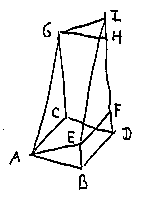
\includegraphics[height=5cm]{2020-2-C3/20210428_C3_exercicio_9.pdf}
 }
$
%

%L rv()
\pu

% Falta:
%\put(3,6.25){\cell{(3,6)}}%
%\put(8,0.75){\cell{(8,1)}}%





\newpage

% «exercicio-6»  (to ".exercicio-6")
% (c3m211dpp 10 "exercicio-6")
% (c3m211dpa   "exercicio-6")

{\bf Exercício 6.}

(Este exercício generaliza as idéias do exercício anterior).

\ssk

Sejam:
%
$$\begin{array}{rcl}
  F &:& \R^2 → \R, \\
  S &=& \setofxyzst{z=F(x,y)}, \\
  A_0 &=& (x_0,y_0), \\
  A &=& (x_0,y_0,F(x_0,y_0)), \\
  \vv &=& \VEC{1,0,F_x(A_0)}, \\
  \ww &=& \VEC{0,1,F_y(A_0)}, \\
  α,β &∈& \R. \\
  \end{array}
$$

a) Identifique no diagrama do próximo slide os pontos:

$A+\vv$, $A+\aa\vv$, $A+\ww$, $A+\bb\ww$, $A+\aa\vv+\bb\ww$, 

Dica: $α$ é aproximadamente 4, e $β$ aproximadamente 2.5.

\newpage

% (find-latexscan-links "C3" "20210428_C3_exercicio_10")
% (find-xpdf-page "~/LATEX/2020-2-C3/20210428_C3_exercicio_10.pdf")
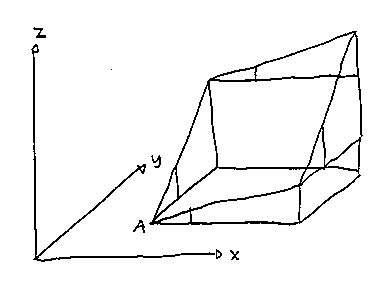
\includegraphics[height=8cm]{2020-2-C3/20210428_C3_exercicio_10.pdf}


\newpage

{\bf Exercício 6 (cont.)}

\msk

b) Verifique -- visualmente -- que os pontos

$A+\vv$, $A+\aa\vv$, $A+\ww$, $A+\bb\ww$, $A+\aa\vv+\bb\ww$, 

do item (a) estão todos no mesmo plano.

\msk

c) Verifique que esse plano é o plano tangente

à superfície $S$ no ponto $A$.




% (c3m202planotangp 10 "geral-e-particular")
% (c3m202planotanga    "geral-e-particular")
% (c3m202planotangp 22 "derivs-como-triangs")
% (c3m202planotanga    "derivs-como-triangs")
% (c3m202planotangp 24 "dicas-6a-e-6d")
% (c3m202planotanga    "dicas-6a-e-6d")



%\printbibliography

\GenericWarning{Success:}{Success!!!}  % Used by `M-x cv'

\end{document}

%  ____  _             _         
% |  _ \(_)_   ___   _(_)_______ 
% | | | | \ \ / / | | | |_  / _ \
% | |_| | |\ V /| |_| | |/ /  __/
% |____// | \_/  \__,_|_/___\___|
%     |__/                       
%
% «djvuize»  (to ".djvuize")
% (find-LATEXgrep "grep --color -nH --null -e djvuize 2020-1*.tex")

 (eepitch-shell)
 (eepitch-kill)
 (eepitch-shell)
# (find-fline "~/2021.1-C3/")
# (find-fline "~/LATEX/2021-1-C3/")
# (find-fline "~/bin/djvuize")

cd /tmp/
for i in *.jpg; do echo f $(basename $i .jpg); done

f () { rm -fv $1.png $1.pdf; djvuize $1.pdf }
f () { rm -fv $1.png $1.pdf; djvuize WHITEBOARDOPTS="-m 1.0" $1.pdf; xpdf $1.pdf }
f () { rm -fv $1.png $1.pdf; djvuize WHITEBOARDOPTS="-m 0.5" $1.pdf; xpdf $1.pdf }
f () { rm -fv $1.png $1.pdf; djvuize WHITEBOARDOPTS="-m 0.25" $1.pdf; xpdf $1.pdf }
f () { cp -fv $1.png $1.pdf       ~/2021.1-C3/
       cp -fv        $1.pdf ~/LATEX/2021-1-C3/
       cat <<%%%
% (find-latexscan-links "C3" "$1")
%%%
}

f 20201213_area_em_funcao_de_theta
f 20201213_area_em_funcao_de_x
f 20201213_area_fatias_pizza



%  __  __       _        
% |  \/  | __ _| | _____ 
% | |\/| |/ _` | |/ / _ \
% | |  | | (_| |   <  __/
% |_|  |_|\__,_|_|\_\___|
%                        
% <make>

 (eepitch-shell)
 (eepitch-kill)
 (eepitch-shell)
# (find-LATEXfile "2019planar-has-1.mk")
make -f 2019.mk STEM=2021-1-C3-derivadas-parciais veryclean
make -f 2019.mk STEM=2021-1-C3-derivadas-parciais pdf

% Local Variables:
% coding: utf-8-unix
% ee-tla: "c3dp"
% ee-tla: "c3m211dp"
% End:
